\chapter{Software Design and Implementation}
\label{chap:software-design}

\section{Background}
This section will provide details of the existing software and services that are leveraged to create the Collaborative Environment. For each, we provide the reasoning for its use as well as a technical description.

\subsection{Symfony}
The Collaborative Environment is built using Symfony Standard Edition, an open-source, object-oriented PHP framework designed around the Model-View-Controller (MVC) software architecture. Using Symfony to create the Collaborative Environment encourages the use of design patterns that are well understood and allows for more of the development time to focus on application features rather than reimplementing standard components of web applications.

The MVC architecture separates an application's business logic, that is, all of the algorithms which process the exchange of data between an interface and a database, from its user interfaces. The \emph{model} consists of object representations of application data (Entities) and a persistence layer, which will store and retrieve entities via a databases management system. The \emph{view} will render a model object into a user interface, such as a web page. The \emph{controller} is what mediates transactions between the user and the application. The typical control flow of a basic MVC application is:

\begin{singlespacing}
\begin{enumerate}
	\item Client makes a request
	\item Controller receives the request and transforms it into a manipulation of the Model
	\item The updated Model is saved to the database by the persistence layer from the Controller
	\item A View is generated by the Controller which makes the changes to the Model visible
	\item The Controller responds to the Client's request with the generated View.
\end{enumerate}
\end{singlespacing}

Symfony Standard Edition comes with many software bundles which extend the core Symfony framework to provide an enterprise-grade application skeleton. Three of the key bundles included are the Security, Doctrine, and Twig bundles, which provide user-rights management, an object-relational mapper, and a template engine respectively.

\subsubsection{Security}
Security in Symfony is handled by a two-step process: authentication and authorization. The authentication step identifies a user and is typically accomplished by having a user first visit the website, at which point they are authenticated as an anonymous user, and then having them provide a set of credentials to authenticate them as a specific user. Authorization occurs when a user attempts to access a resource of an application. Symfony allows for a set of user roles to be defined, of which each user has a set of, as well as an access control list, to determine exactly what resources any given user has access to.

Controllers are aware of what the current user's authentication is and, as such, can be configured to only allow processing to occur if and only if the current user has a given role. While an Entity will generically describe all instances of a piece of data in an application, if the currently authenticated user should only have access to an exact instance of an entity, an entry can be added to an access control list for that particular user-entity instance pair.

These features provide the Collaborative Environment with a powerful and robust mechanism that is essential to securing the Student data being tracked.

\subsubsection{Doctrine}
In a dynamic web application, Entities are constantly being created, read, update, and deleted. To keep track of these changes, it is natural to consider using a database management system (DBMS) such as MySQL or PostgreSQL. In an object-oriented program, these Entities often contain non-scalar data (e.g. lists, arrays) that must be persisted by a DBMS, which can be problematic because a DBMS can often only store scalar data (e.g. strings, integers). Using an object-relational mapper (ORM), such as Doctrine, solves this problem by managing the transformation to and from scalars/non-scalars when persisting an object.

As an example of how an ORM operates, let's consider an object-oriented system where a Student is enrolled in a set of Courses. Naturally, we would have two Entity objects, Student and Course. The fields of the Student entity could be an ID, a name, and a list of Courses that they're enrolled in (consider this to be a many-to-many relationship). The fields of the Course Entity could be a name and number. When a new Student has been created and they are enrolled in, perhaps, two different Courses and the ORM is told to persist this data, it will store the scalar data in the  DBMS as its native types (names map to varchar, IDs and numbers map to integer), but for the Student's list of enrolled courses, since we established that there is a many-to-many relationship, the ORM will manage a Student ID-Course number tuple (Student 1 is enrolled in Course 1, Student 1 is enrolled in Course 2). Of course, when this data is requested from the DBMS, the ORM will convert the data back into Entity objects.

\subsubsection{Twig}
When a Controller has to return a new response, it is common for the View to be defined as a template that will be rendered though an engine, such as Twig, rather than explicitly crafted in the desired output format. For example, this could be accomplished by designing a Twig template that will output specific Model Entity variables and have it be processed into HTML by the Twig engine instead of just writing a mixture of HTML and PHP directly.

There are many benefits to using a template engine, such as:

\begin{description}
	\item [Template inheritance] Defining a parent or a layout template that can be inherited from children allowing for a consistent theme across an application.
	\item [Syntax] Provides numerous shortcuts for applying common patterns to variables such as escaping output and modifying control flow.
	\item [Speed] After compiling a template, the result will be optimized and low-overhead PHP when compared to freehand coding.
\end{description}

\subsection{Khan Academy}
The Khan Academy is a nonprofit organization that aims to better global education by providing free, high-quality resources to anyone anywhere. \cite{khan-website-about} On their website, they provide in excess of 2700 videos that teach varying topics in STEM fields. The organization has been provided with the financial support and public accolades of large entities such as The Bill \& Melinda Gates Foundation and Google \cite{khan-wiki-sources} indicating that they produce noteworthy content. The videos that Khan Academy hosts are all created by Salman Khan who holds an MBA from Harvard and three science degrees from MIT. Each is produced in a fairly consistent manner using a software whiteboard, a screen capture program, and a microphone while typically lasting about 10 minutes.

As stated in \S \ref{sec:overview-goals} and \S \ref{sec:overview-features}, students using the Collaborative Environment should have access to supplemental learning resources and will have the ability to take quizzes given by their teachers and teaching assistants. The Khan Academy videos are ideal for this use as they are concise and short enough to be associated with individual quizzes that are created in the Collaborative Environment. If a student, while taking a quiz, feels that they are in need of some assistance, a link to the an appropriate Khan Academy video will be readily available to them.

\section{Features}
\label{sec:features}
We now describe the main features of the Collaborative Environment as previously outlined in \S \ref{sec:overview-features}. Each subsection henceforth provides the concept, design, and implementation of an individual feature. They have been arranged in such a way that each successive feature will build on the previously introduced ones.

%%%% Academic
\subsection{Academic Year}
\label{subsec:design-year}
In a traditional document-based teaching environment, student data is stored in numerous grade books  or spreadsheets which are held by many different people in many different places. Each teacher, for instance, would have their own set of student records and a district will have a permanent record for each student containing information such as their standardized test scores. If an administrator managed to collect all of this data into a single place, however frustrating that may be, the next thing they would have to do to it, before any type of analysis, would be to group it all by what year the record corresponds to.

As the Collaborative Environment will be collecting data year after year, an Academic Year entity is required. Teachers, Teaching Assistants, and Students all have data associated with them that can change on an annual basis. Students will be taking different classes, have taken different standardized tests, and participated in different activities as well as be in a different grade altogether or have graduated. Each year can also bring with it a different round of quizzes and surveys and even new Teachers or Teaching Assistants.


\subsubsection{Design}
The Year entity is really very simple, just a primary key identifier, \emph{id}, and the year itself as an integer, \emph{year}. Explicitly storing the years that the Collaborative Environment will be tracking in a table allows consistency throughout the entire application and customization by an administrator. An alternative implicit design would have been to keep a \emph{date} column in each entity that was going to have time-sensitive content added to it and the server would be responsible for getting the current year from the operating system, but problems arise if the system's time and date are not correct. 

\begin{figure}[h!]
	\centering
	\fbox {
		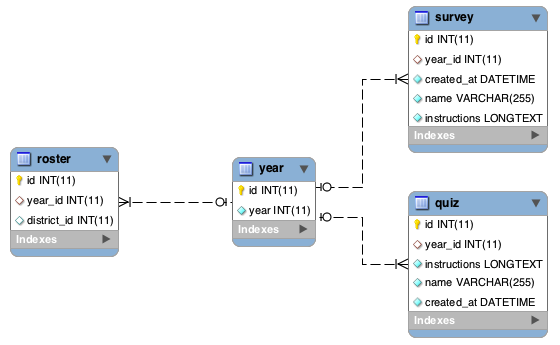
\includegraphics[width=0.7\textwidth]{figures/er/year}
	}
	\caption{Year Enhanced Entity-Relationship (EER) Diagram}
	\label{fig:er-year}
\end{figure}

We see in Figure \ref{fig:er-year}, that the year entity appropriately maintains a one-to-many relationship with each of the tables that reference it. In an EER diagram such as this, each box represents a table in a database and each row in a box corresponds to a column in that table. A connecting line indicates that a relationships exists between its connected tables. If we take the relationship between the year and survey tables as an example, the line, which is drawn using Crow's Foot notation, indicates that a survey can be given during one year and that a year can have many surveys given during it. This diagram additionally indicates that many quizzes (see \S \ref{subsec:design-quiz}) and many rosters (see \S \ref{subsec:design-district}) can also only be associated with only one year.

The user's choice of which year they want to have as their current context for data viewing and manipulation will have to persist between each page of the Collaborative Environment. Having to constantly select what year to interact . Therefore, once a user initially visits the web site, a PHP session variable will be established that tracks the year they select which will then be used by subsequent SQL queries to retrieve the requested data.

\subsubsection{Implementation}
As established in the previous section, the selected year must be persisted from page-to-page as well as be accessible in such a way that it will not require a user to constantly have to interact with a selector.

This was implemented by having a year selector list appear in the upper-right corner of each page in the Collaborate Environment, as shown in Figure \ref{fig:screens-year}. The list is populated by making an asynchronous HTTP GET request to the URL \texttt{/year} which will both provide all available academic years that have been configured and indicate which is the current year as selected by the user.

\begin{figure}[h!]
	\centering
	\fbox{
		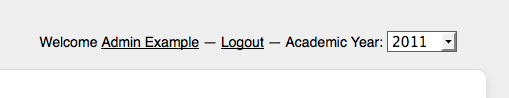
\includegraphics[width=0.6\textwidth]{figures/screens/year}
	}
	\caption{Year Selector Highlight}
	\label{fig:screens-year}
\end{figure}

Upon choosing a year from the selection, if it differs from the currently selected year, then an HTTP POST request will be sent to \texttt{/year/change/\textit{selected-year}}. This will cause the year PHP session variable to be updated to \emph{selected-year}. If the server responds with a success message, then the current web page will be refreshed and any changes to the data that are dependent on the year will be reflected.

%%%% Users
\subsection{User Management}
\label{subsec:design-user}
A User entity is perhaps the most fundamental object in the Collaborative Environment.  Users of each class, as defined in \S \ref{sec:overview-user-classes}, with the exception of anonymous, will be required to have an account with this system, and that account is what the User entity represents. The set of users minus anonymous will be referred to as ``registered users''.

	This entity facilitates the fulfillment of the Collaborative Environment's goal of logging user data by allowing the storage of a student's personal data such as gender, ethnicity, if they've graduated, and what college they are attending, in addition to student educational data such as standardized test scores, courses enrolled in, and after-school activities.

The collaborative functionality of the system also requires a User entity. Quiz attempts, survey submissions, and messaging need a way of differentiating one user from another.

\subsubsection{Design}
The Collaborative Environment internally refers to the set of user classes as ``roles''. Roles are easily stored in the database by using a role table such that its \emph{name} is stored in a column. The User entity, as modeled in Figure \ref{fig:er-user} stores two types of data: required information that applies to all registered users and personal/educational data that applies strictly to students. Required information consists of a user's \emph{username}, \emph{password}, \emph{salt}, \emph{firstName}, and \emph{lastName}.

\begin{figure}[h!]
	\centering
	\fbox{
		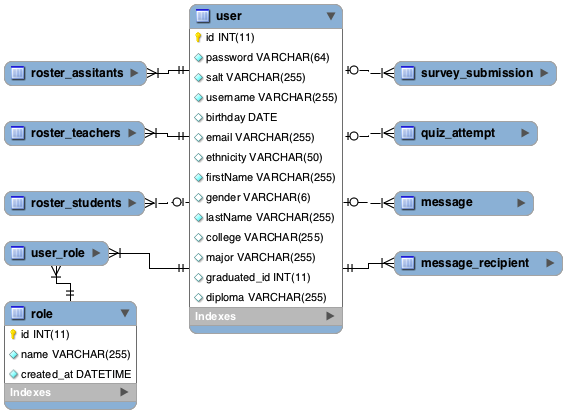
\includegraphics[width=0.7\textwidth]{figures/er/user}
	}
	\caption{User and Role EER Diagram}
	\label{fig:er-user}
\end{figure}

Each of these attributes has an obvious use except, perhaps, for \emph{salt} which is a precautionary security measure. All user passwords are hashed using using the SHA-256 cryptographic hash function. This means that if two users had the same password, then they would obviously result in identical hashes. This fact can be used exploited by people that have large masses of precomputed hashes. A salt, which is a randomly generated string, is append to the plaintext of a password before it is hashed. Now, even if the user's password is something common, what is hashed is, most likely, something unique.

For the sake of simplicity, we decided that the personal/education attributes \emph{birthday}, \emph{email}, \emph{ethnicity}, \emph{gender}, \emph{college}, \emph{major}, \emph{diploma}, and \emph{graduated} as year-independent data. This means that if and when these attributes have a value, that it will not vary based on what academic year the client has selected to be the current year; their values will persist through all years. On the other hand, there is strictly educational data that we do treat as year-dependent: activities, courses, exams, and grade level.

\begin{figure}[h!]
	\centering
	\fbox{
		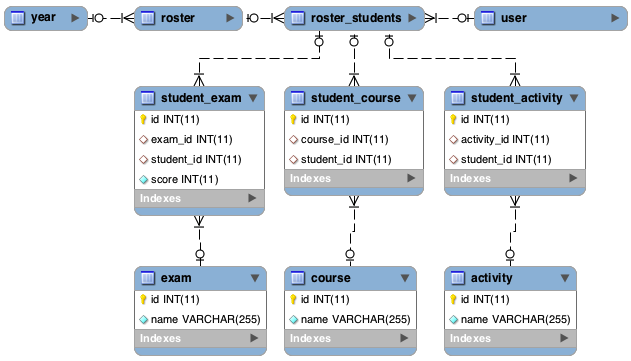
\includegraphics[width=0.7\textwidth]{figures/er/user-student}
	}
	\caption{Student user EER Diagram}
	\label{fig:er-user-student}
\end{figure}

Figure \ref{fig:er-user-student}, outlines the general model to achieve a year-dependent relationship between a student and their educational data and will be explained in depth in \S \ref{subsec:design-district}. Any given year is associated with many rosters, each of which contain a set of students in varying grade levels. Each student in a roster can then be associated with many exams, courses, and activities. 

\subsubsection{Implementation}
User management is broken up into three processes: creation, updating, and reading. As an interface to each of these processes, privileged users have access to a user management interface seen in Figure \ref{fig:screens-user-list}. This interface will only display the users that the currently authenticated user has access to. For administrators, this will be all users, whereas a teacher or a teaching assistant will only see the students that belong to the district that themselves belong to. For example, if a teacher is listed as being a teacher in the district ``Public School \#1'' for the year 2011, then the user list will only show students that also enrolled at the district during that year.

This idea of teachers and teaching assistants only having access to the students that are on the same roster as them is persistent throughout the application. The details regarding districts, rosters, and permissions will be explained in \S \ref{subsec:design-district}.

With this data now being tracked by the Collaborative Environment, trends and reports will be able to be generated. Tracking student participation in activities, courses, and exams is now possible for the set of all students or even subsets such as minorities, males, or females.

\begin{figure}[h!]
	\centering
	\fbox{
		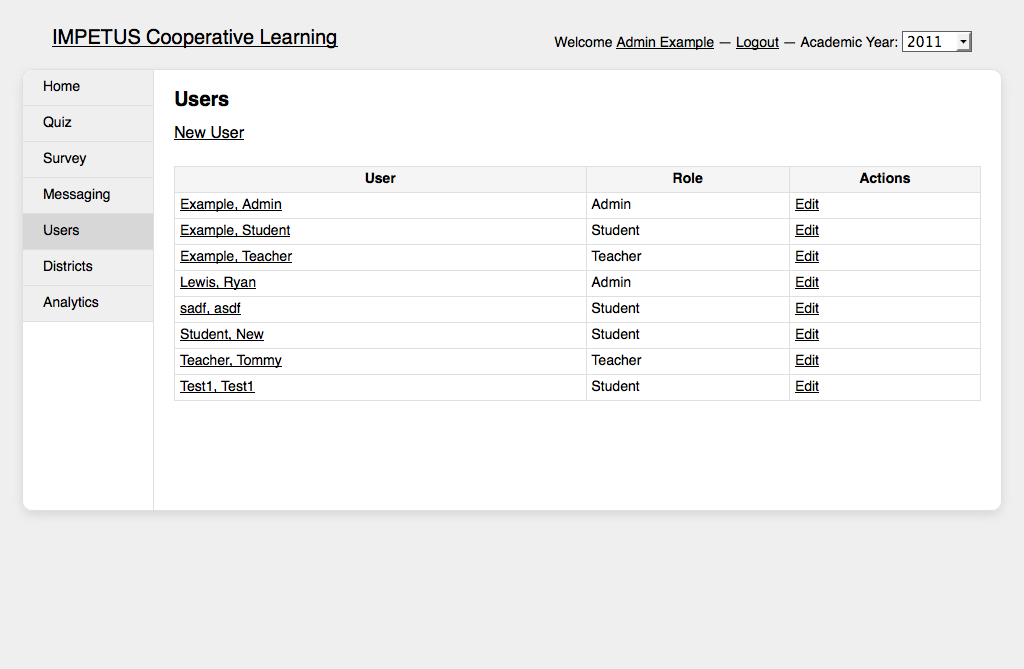
\includegraphics[width=0.8\textwidth]{figures/screens/user-list}
	}
	\caption{A privileged user's view of all the system's users.}
	\label{fig:screens-user-list}
\end{figure}

When a privileged user must add or edit a user, the interface appears as it does in Figure \ref{fig:screens-user-student-edit}, except all of the fields are simply blank in the case of adding a new user. The interface has has been split horizontally into two sections, the top is for personal/educational data whereas the bottom is for strictly educational data. In the top half, input fields has been grouped into sets of required and supplemental (optional). This allows the user to readily identify which fields they must have a value for and not have to wait for the program to return an error.

\begin{figure}[h!]
	\centering
	\fbox{
		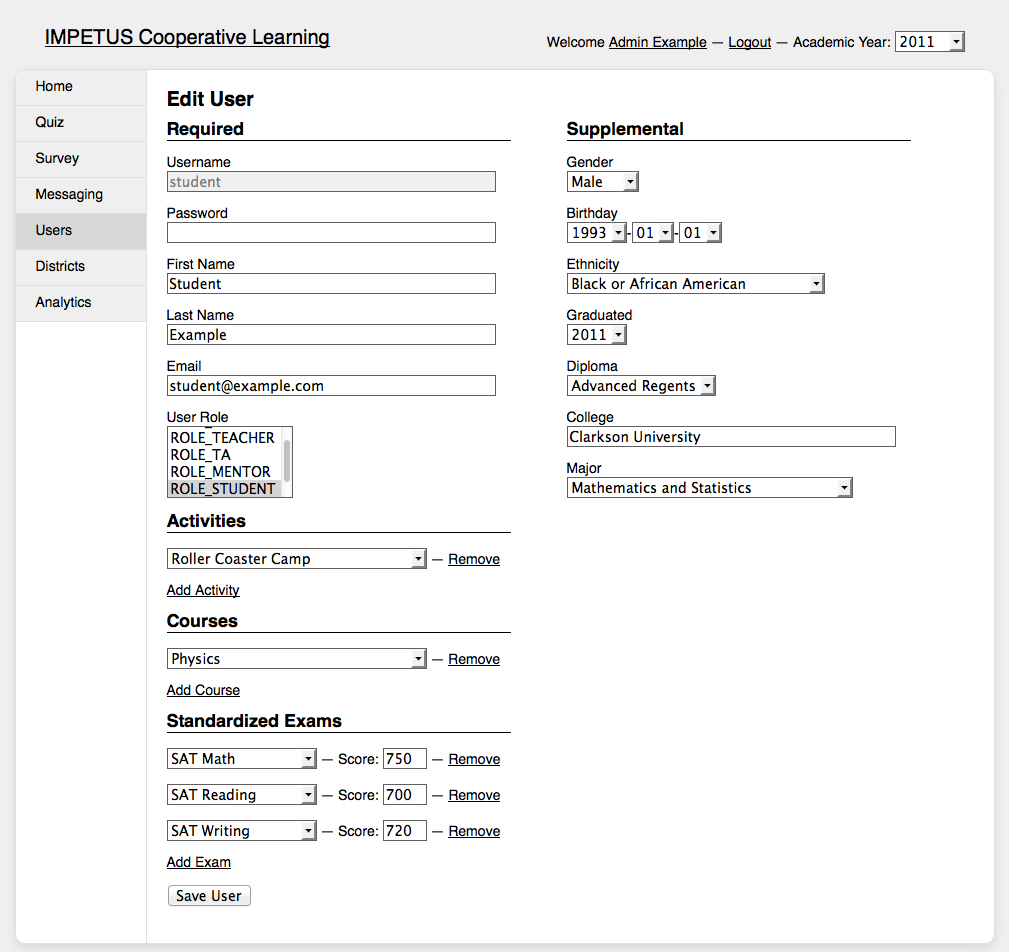
\includegraphics[width=0.8\textwidth]{figures/screens/user-student-edit}
	}
	\caption{A privileged user editing a student's account.}
	\label{fig:screens-user-student-edit}
\end{figure}

The supplemental fields for \emph{ethnicity}, \emph{diploma}, and \emph{major}, provide the user with a limited selection of options rather than a freely fillable text input because this will allow for consistent data analysis. If users were able to enter whatever they wanted for these, it would become difficult to use that data to generate accurate reports. For example, if one person were to enter that a student was going to major in ``Mathematics'' and another were to enter ``Math''.

Since the bottom half of the screen only applies to students, where strictly educational data is entered, it will only appear if the user is assigned the Student role. As stated in the Implementation section, \emph{activities}, \emph{courses}, and \emph{exams} are year-dependent. This means that if a user were to choose different academic years while editing a student's data, they would see these fields change appropriately. A student can be associated with as many year-dependent  fields as necessary by clicking the Add button for the appropriate section.

Lastly, viewing user data in a more organized fashion is shown in Figure \ref{fig:screens-user-student-profile}. This simply provides an view into the data stored for a user. Just as the add/edit screen would update its data when the current academic year is changed, so will the view screen.

\begin{figure}[h!]
	\centering
	\fbox{
		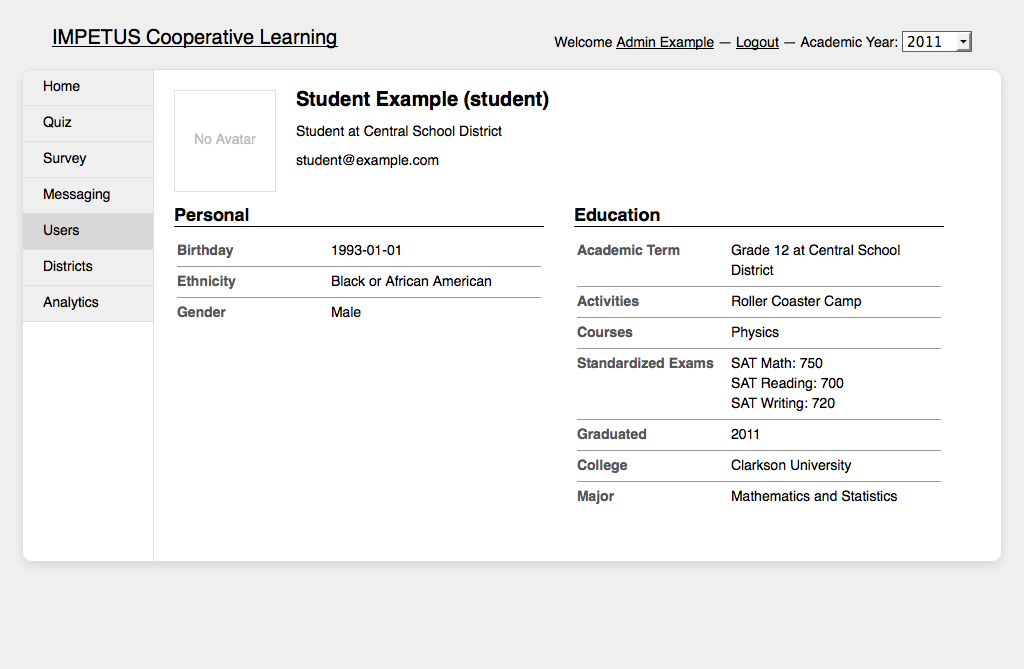
\includegraphics[width=0.8\textwidth]{figures/screens/user-student-profile}
	}
	\caption{A privileged user's view of a student's profile.}
	\label{fig:screens-user-student-profile}
\end{figure}


%%%% Districts
\subsection{District Management}
\label{subsec:design-district}
test

\begin{figure}[h!]
	\centering
	\fbox{
		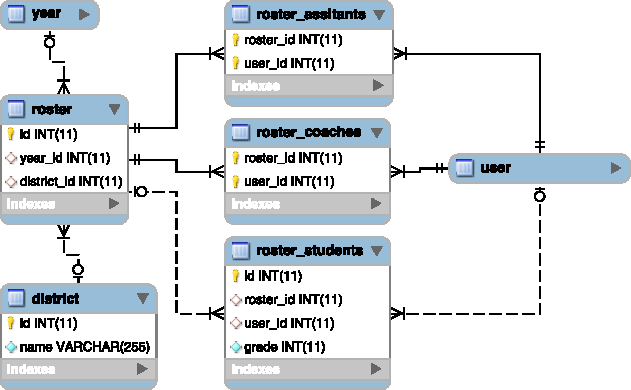
\includegraphics[width=0.7\textwidth]{figures/er/district.pdf}
	}
	\caption{District and Roster EER}
	\label{fig:er-district}
\end{figure}



\begin{figure}[h!]
	\centering
	\fbox{
		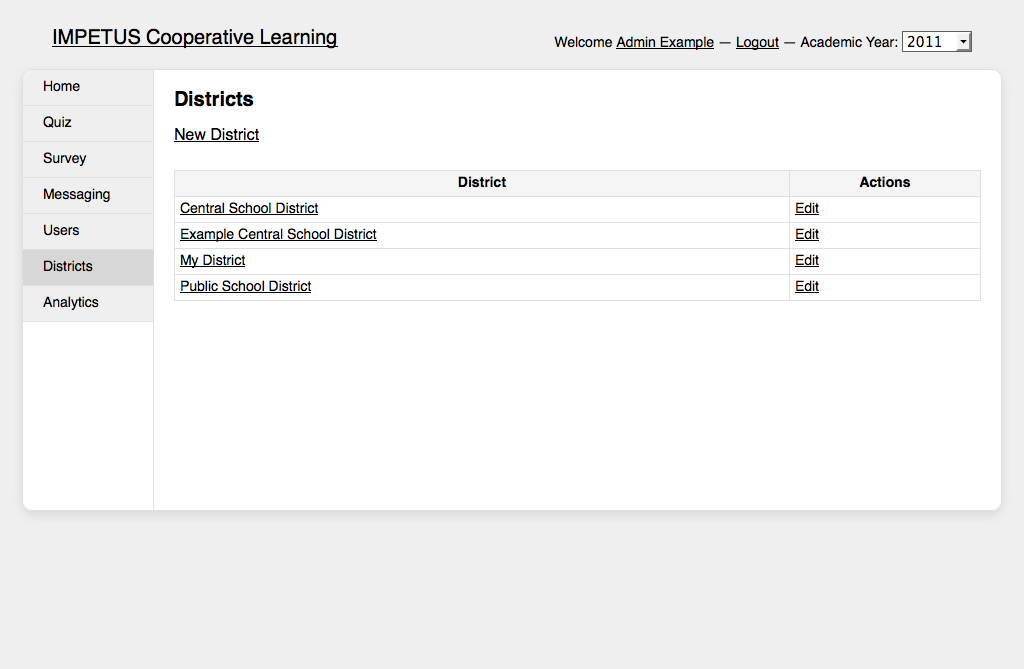
\includegraphics[width=0.8\textwidth]{figures/screens/district-list}
	}
	\caption{A privileged user's view of all the system's users.}
	\label{fig:screens-district-list}
\end{figure}



\begin{figure}[h!]
	\centering
	\fbox{
		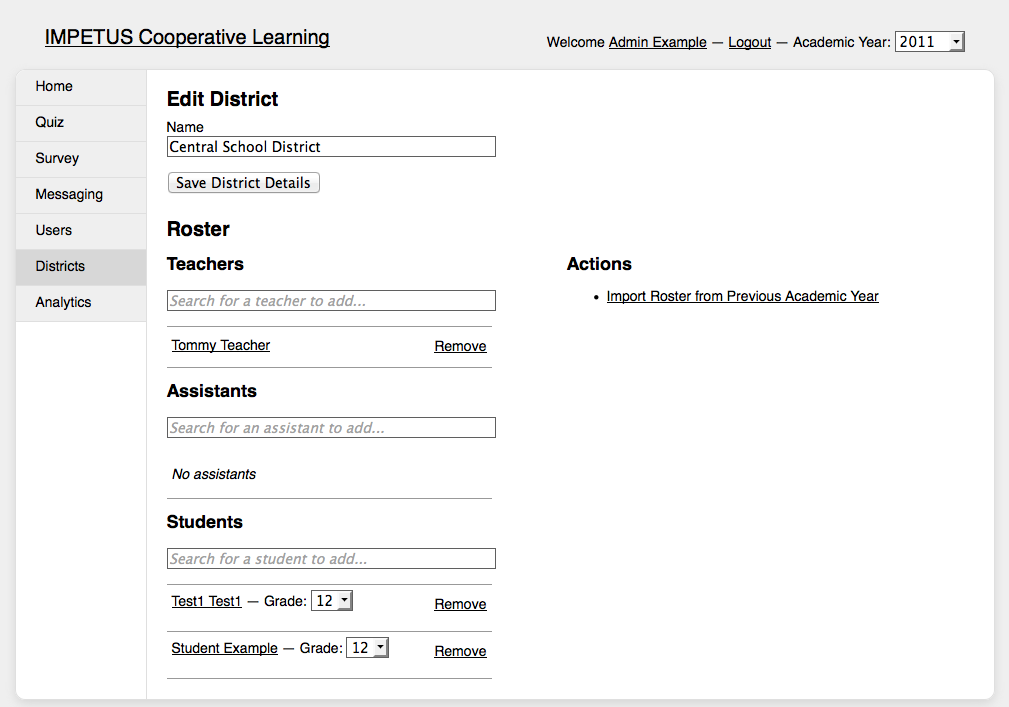
\includegraphics[width=0.8\textwidth]{figures/screens/district-edit}
	}
	\caption{A privileged user editing a district.}
	\label{fig:screens-district-list}
\end{figure}


%%%% Quiz
\subsection{Quiz System}
\label{subsec:design-quiz}
test

%%%% Survey
\subsection{Survey System}
\label{subsec:design-survey}
test

%%%% Messaging
\subsection{Messaging}
\label{subsec:design-messaging}
test

%%%% Analytics
\subsection{Analytics}
\label{subsec:design-analytics}
test

\section{Known Issues}